\documentclass[
    parskip=half, 
    twoside=false,
    twocolumn=true,
    fontsize=11pt,
]{scrarticle}
\input{../preamble.tex}
\addbibresource{literature.bib}

\begin{document}

\title{title}
\subtitle{subtitle}
\author{Aurel Müller-Schoenau, Leon Oleschko}
\date{\dotdate\today}


% make a custom title page
\begin{titlepage}
    \sffamily
    \vspace*{3cm}
    {
        \fontsize{32}{32}
        \markieren{}{}{Earth Field}{Nuclear Magnetic Resonance}
    }
    \vspace{.25cm}\\
    {
        \Large
        Aurel Müller-Schoenau, Leon Oleschko\\
        Supervised by Stefan Kraner
        \vspace{.05cm}\\
        18.12.2024
        \vspace{.25cm}\\
        \normalsize
        Physikalisches Fortgeschrittenenpraktikum 2\\
        Universität Konstanz
    }
    \vfill
    {
        \normalfont\normalsize 
        TODO
    }
    \vfill
    \begin{flushright}
        Available at \url{www.github.com/leoole100/fp2}.
    \end{flushright}
\end{titlepage}

\section{Introduction}

\section{Find Section Title}

The key principle behind the Nuclear Magnetic Resonance measurement is that a nucleus that posesses a magnetic moment which is not aligned with an external magnetic field will rotate around the magnetic field axis at its \textit{Larmor Frequency}
\begin{equation}
\label{eq:larmor_frequency}
 \omega = \gamma B
\end{equation}
where $B$ is the magnetic flux density and $\gamma$ is the gyromagnetic ratio of the nucleus. If many nuclei oscillate coherently, the corresponding magnetic moment can be detected externally.\\
In order to achieve coherence throughout the sample, the field strength $B$ must not vary significantly with position. For this experiment, the earths magnetic field is sufficient and will serve as the external field. This method is called \textit{Earth Field Nuclear Magnetic Resonance}.


\subsection{Noise Analysis}
\begin{figure}[h]
    \centering
    \label{fig:tune_C}
    \includegraphics{figures/01 noise.pdf}
    \caption{TODO}
\end{figure}

To detect the signal later during the experiment, an electric resonant circuit of the same resonant frequency $\omega$ will be brought close to the sample. Such a circuit contains an inductance $L$ represented by a coil in the center of which the sample is located; the coil acts as the detector for the oscillating magnetic moment. A capacitor with capacitance $C$ and an ohmic resistor $R$ connected in series with the coil create an LCR circuit. Current $I$ and voltage $U$ follow a specific relationship in each of the components. For the whole circuit, this results to a second-order differential equation for $I$ and $U$ equivalent to that of a harmonic oscillator with a resonance frequency of
\begin{equation}
 \label{eq:LCR_frequency}
 \omega_{\text{LCR}} = \frac{1}{\sqrt{LC}}
\end{equation}
Given the detector coil of fixed inductance $L$, a variable capacitor can be used to tune the circuit to the larmor frequency of the sample. \autoref{fig:tune_C} shows the noise magnitude detected by the circuit with respect to variable resonant frequency following a change in $C$. The spectrum consists of a noise floor below \SI{0.1}{\micro \volt \per \hertz}, a large peak around \SI{2}{\kilo \hertz} at \SI{0.5}{\micro \volt \per \hertz} as well as a series of spikes at uneven multiples of roughly \SI{50}{\hertz}. Those spikes are likely caused by the power supply connected to the grid. The large spike might be the mechanical resonance frequency of the coil, because the magnitude increased a lot when playing a \SI{2}{\kilo \hertz} tone next to it. All other noise sources, like lamps or electronic devices, and the noise generated in the measurement electronics, add up to the remaining noise floor.


\subsection{Free Induction Decay}
\begin{figure}[h!]
    \centering
    \includegraphics{figures/02 fid.pdf}
    \caption{TODO}
\end{figure}

\subsection{Spin Lattice Relaxation}
\begin{figure}[h!]
    \centering
    \includegraphics{figures/03 T1.pdf}
    \caption{TODO, $T_1 = \SI{2.003(27)}{s}$}
\end{figure}

\subsection{Spin Echo}
\begin{figure}[h!]
    \centering
    \includegraphics{figures/04 spin echo shims.pdf}
    \caption{TODO}
\end{figure}

\subsection{Multiple-echo experiments}
\begin{figure*}[h!]
    \centering
    \includegraphics{figures/05 CPMG.pdf}
    \caption{TODO}
\end{figure*}

\subsection{Relaxation Time Contrast}
\begin{figure}[h!]
    \centering
    \includegraphics{figures/06 contrast.pdf}
    \caption{TODO}
\end{figure}

\subsection{Imaging}
\begin{figure*}[h!]
    \centering
    \begin{subfigure}[c]{.45\textwidth}
        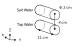
\includegraphics{figures/07 sample holder.pdf}
        \caption{TODO}
    \end{subfigure}
    \begin{subfigure}[c]{.45\textwidth}
        \includegraphics{figures/07 1d imaging.pdf}
        \caption{TODO}
    \end{subfigure}
    \caption{}
\end{figure*}

\begin{figure*}[h!]
    \centering
    \includegraphics{figures/08 2d imaging.pdf}
    \caption{TODO}
\end{figure*}


\section{Conclusion}

\addcontentsline{toc}{section}{Literature}
\nocite{*}
\printbibliography

\end{document}
